\section{Discussion}
\label{sec:discussion}

\subsection{Recurrent Warm-Up Latency}
\label{sec:disc:warmup}

A finding not discussed in the original \fastgrnn{}
paper~\cite{kusupati2018fastgrnn} is that prediction stability
requires a non-trivial number of samples of hidden-state
evolution before the emitted class label settles,
regardless of the underlying deployment target. Fig.~\ref{fig:warmup}
traces the emitted label and the $h_0$ component over a single
\textsc{standing} window: the model passes through \textsc{walking}
and \textsc{upstairs} predictions before locking onto the correct
class. This is a property of the recurrent
dynamics, not of either MCU; both Arduino and MSP430 produce
identical trajectories (Section~\ref{sec:results:crossplatform}).

To quantify the distribution, we evaluated 100 randomly sampled test
windows using the deployed seed-0 model and measured, for each window,
the first step $t^*$ at which the per-step prediction matches the
final-window prediction and remains stable for all subsequent steps.
The \textbf{median stabilization point is 74 samples (1.48~s)},
with an IQR of 40--86 samples (0.79--1.72~s) and a worst-case of
125 samples (2.50~s at 50~Hz).

For user-facing applications -- fall detection, gesture recognition,
posture coaching -- this implies that activity \emph{transitions}
are confirmed with a median latency of $\sim$1.5~s and a worst-case
of $\sim$2.5~s after they occur. This is a non-trivial latency budget
and should be reported alongside per-sample throughput when
characterizing on-device RNNs. We hypothesize the same effect occurs
in other gated recurrent cells of comparable size; verifying this on
LSTM/GRU baselines at matched parameter counts is an obvious
follow-up.

\begin{figure}[t]
\centering
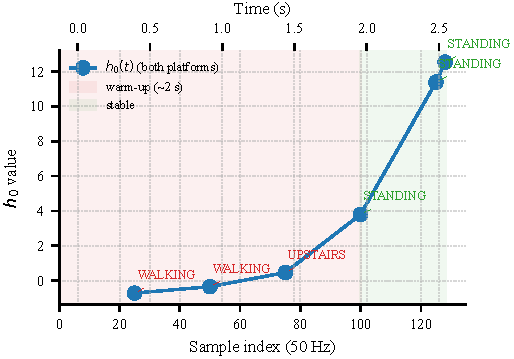
\includegraphics[width=\linewidth]{figures/warmup_curve.pdf}
\caption{Hidden-state component $h_0$ and emitted class label over
a single 2.56~s window (50~Hz, \textsc{standing} ground truth).
Both Arduino and MSP430 produce identical trajectories. The class
label is unstable during the recurrent warm-up; over 100 random
test windows the median stabilization point is 74 samples (1.48~s),
with a worst-case of 125 samples (2.50~s).}
\label{fig:warmup}
\end{figure}

\subsection{Cross-Platform Determinism as Reproducibility}
\label{sec:disc:determinism}

Modern ML inference is frequently non-reproducible across hardware
due to vendor-specific BLAS, mixed-precision tensor cores, and
non-associative floating-point reductions. By contrast, our
portable C engine -- using software-emulated floating-point on
both 8-bit AVR and 16-bit MSP430 targets -- produces \emph{bit-equivalent}
predictions across platforms (Section~\ref{sec:results:crossplatform}).
This level of determinism is itself an artifact worth preserving
in safety-relevant deployments such as medical-grade HAR, where
regulatory bodies increasingly require that a software change be
re-validated only against the exact hardware on which it was
qualified. A bit-equivalent inference path across two different
ISAs is a useful escape hatch from that constraint.

\subsection{Headroom Analysis and the Pure-Q15 Dead End}
\label{sec:disc:headroom}

The \msp{} consumes 65\% of the 20~ms budget per sample, leaving
$\sim$7~ms of headroom (Section~\ref{sec:results:streaming}). In
live MPU-6050 testing this headroom comfortably absorbs an
I\textsuperscript{2}C accelerometer read, an LED status update,
and a UART log line per sample.

We did briefly explore a more aggressive \emph{pure-Q15} inference
path -- weights, activations, \emph{and} intermediate products all
in Q15 integer arithmetic. The pipeline failed empirically: the
chained per-tensor scales attenuate to $\sim$$10^{-13}$ over the
multi-stage low-rank product, which is unrepresentable in a Q15
multiplier without an int64 accumulator and a custom per-stage
shift schedule. Replacing the per-tensor scales with the simpler
fixed Q9.6 format discussed in Section~\ref{sec:method:q15}
alleviates the chaining problem but reintroduces it on the
weight side: weight magnitudes span four orders of magnitude
across tensors, so a uniform Q9.6 scale wastes up to $8\times$
of weight resolution per tensor relative to the calibrated path.
The clean fix is quantization-aware training~\cite{hubara2017qnn},
which constrains the scale schedule during training rather than
discovering it post-hoc. Given that
the LUT-based FP32 path already meets the 50~Hz real-time
constraint with comfortable headroom, we did not pursue the
QAT approach in this work; we revisit it as future work in
Section~\ref{sec:disc:future}.

\subsection{Limitations}
\label{sec:disc:limitations}

Three limitations bound the scope of our claims:

\begin{itemize}
\item \textbf{Dataset.} \hapt{} is recorded under laboratory
conditions with a fixed waist-mounted smartphone. On-body sensor
displacement, free-living data distribution shift, and
inter-subject variation are known to degrade HAR
accuracy~\cite{wang2019harsurvey,demrozi2020harsurvey} and are not
modelled here.

\item \textbf{Label set.} We train and evaluate on the six basic
\hapt{} activities. The full \hapt{} label set adds six postural
transitions (e.g.\ \textsc{stand-to-sit}, \textsc{lie-to-sit})
which our model does not handle. This is a deliberate choice
to match the original \fastgrnn{} HAR benchmark.

\item \textbf{The DOWNSTAIRS class.} \textsc{downstairs} is the
binding-constraint class throughout the pipeline
(Fig.~\ref{fig:perclass}), and we did not attempt class-specific
remediation in this paper. Section~\ref{sec:disc:future} sketches
several plausible interventions.

\item \textbf{Statistical significance testing.} Our multi-seed
evaluation reports mean$\pm$standard deviation across five seeds
but does not include paired significance tests or non-parametric
bootstrap intervals. Formal significance testing is left for
future work.
\end{itemize}

\subsection{Future Directions}
\label{sec:disc:future}

Four extensions are natural next steps from this work.

\begin{itemize}
\item \textbf{Dual-rank static-vs-dynamic decomposition.} In our
rank sweep (Section~\ref{sec:results:lowrank}), $r_u{=}4$ is
favorable for the dynamic classes (\textsc{walking},
\textsc{upstairs}, \textsc{downstairs}) and $r_u{=}8$ is favorable
for the static classes (\textsc{sitting}, \textsc{standing}).
A simple low-cost variant -- $\mathbf{U}_\text{eff} = \mathrm{LowRank}(r{=}4) + \mathrm{diag}(\boldsymbol{\alpha})$
-- adds only $H$ extra parameters while letting a static
DC-like signal pass through the diagonal residual and a dynamic
pattern through the low-rank branch. We expect this to recover
the dynamic-class accuracy of $r_u{=}4$ without the static-class
degradation.

\item \textbf{DOWNSTAIRS-targeted features.} The standard
UCI~HAR pipeline applies a Butterworth low-pass at 0.3~Hz to
separate gravity from body acceleration; we omitted this step to
match the original \fastgrnn{} HAR setup. Re-introducing it, or
augmenting the input with a small number of FFT-band features over
the 128-sample window, is the lowest-cost path to closing the gap
on the \textsc{downstairs} class.

\item \textbf{Quantization-aware training for pure-Q15 inference.}
As discussed in Section~\ref{sec:disc:headroom}, post-training
quantization fails for a fully integer pipeline because of scale
chaining; QAT~\cite{hubara2017qnn} should resolve this. A pure-Q15
path would likely yield an additional 2--3$\times$ speedup on the
\msp{} and is the natural successor to the LUT trick.

\item \textbf{Transition states.} Adding the six postural transitions
of the full \hapt{} label set raises the practical question of
how to allocate the recurrent state between long-horizon
activity recognition and short-horizon transition detection.
A multi-scale recurrent cell, evaluated at two cadences, is a
straightforward starting point.
\end{itemize}
